% basic documentclass
\documentclass[12pt]{book}

% include third party
\usepackage{ctex}
\usepackage{fancyhdr}
\usepackage{graphicx} %插入图片的宏包
\usepackage{float} %设置图片浮动位置的宏包
\usepackage{subfigure} %插入多图时用子图显示的宏包
\usepackage{hyperref}
\usepackage{geometry}

\geometry{right=2.0cm, left=2.0cm}

%% for language
\usepackage{listings}
\usepackage{xcolor}
\lstset { %
	language=C++,
	backgroundcolor=\color{black!5}, % set backgroundcolor
	basicstyle=\footnotesize,% basic font setting
}


% redefine fun
\newcommand{\icenter}[1]{\begin{center}{#1}\end{center}}
\newcommand{\isection}[1]{\begin{center}\section*{#1}\end{center}}

% basic setting
\pagestyle{fancy}

\fancyhead{}
\fancyhead[CE]{My Road To Deep Learning}
\fancyhead[CO]{\leftmark}

% title name
\title{My Road To Deep Learning}
\date{}

% document begin
\begin{document}
	
\maketitle
\thispagestyle{empty}

\newpage
\setcounter{page}{1}

%\fancyhead{}
%\fancyhead[CO,CE]{目录}

\icenter{\tableofcontents}

%%%%%%%%%%%%%%%%%%%%%%%%%%%%%%%%%%%%%%%%%%%%%%%%%%%%%%%%%%%%%%%%%%%%%%%%%%%%%%%%%%%%%%%%%%%%%%%%%%%%%%%%%
%%  第一章 绪论  %%

\newpage

\fancyhead{}
\fancyhead[CO,CE]{绪\ 论}

%\isection{第一章\ 绪\ 论}
\chapter{第一章\ 绪\ 论}
\section{一级标题}
\subsection{二级标题}
\subsection{三级标题}

\section{一级标题}

\noindent TODO:\\1. 

\newpage
this is test
 
 %%%%%%%%%%%%%%%%%%%%%%%%%%%%%%%%%%%%%%%%%%%%%%%%%%%%%%%%%%%%%%%%%%%%%%%%%%%%%%%%%%%%%%%%%%%%%%%%%%%%%%%%%
 %%  第二章 数学基础  %%
 \newpage
 
 \fancyhead{}
 \fancyhead[CO,CE]{数学基础}
 
 %\setcounter{chapter}{0}
 \chapter{第二章\ 数学基础}
 
 %\stepcounter{chapter}
 \section{高斯分布}
 一维的高斯分布(Gaussian distribution)函数表示为:
 \begin{equation}\label{eq:1d-gaussian-distribution}
G(x)=\frac{1}{\sqrt{2\pi }\sigma }e^{-\frac{(x-\mu)^{2}}{2\sigma ^{2}}}
 \end{equation}
其中$\mu$表示均值(mean),$\sigma$表示标准差(standard deviation)。一般用标准差的平方$\sigma^2$来表示方差(variance)。均值表示所有数据的平均值大小,标准差则表示数据和均值之间的偏差程度。假设所有的$N$个数据为$x_1, x_2, ..., x_n$,则均值计算方式为:
\begin{equation}\label{eq:1d-gaussian-distribution-mean}
\mu =\frac{1}{N}\sum_{i=1}^{n}x_i
\end{equation}
标准差的计算公式为:
\begin{equation}\label{eq:1d-gaussian-distribution-var}
\sigma =\sqrt{\frac{\sum \left |  x-\mu \right |^2}{N}}
\end{equation}

\begin{figure}[H]
	\centering
	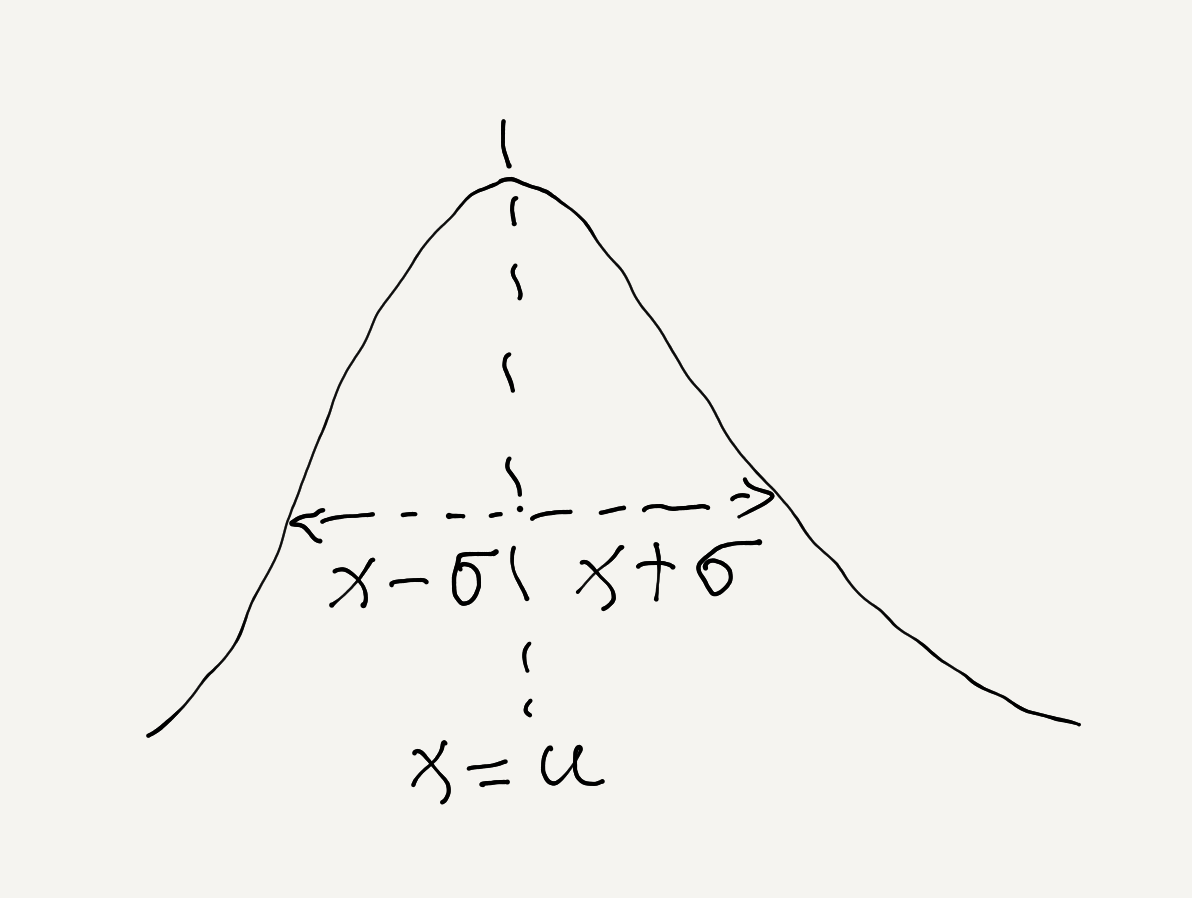
\includegraphics[width=0.7\textwidth]{images/gaussian-distribution.png}
	\caption{高斯分布函数}
	\label{gaussian-distribution} 
\end{figure}

二维高斯分布函数表示为:
 \begin{equation}\label{eq:1d-gaussian-distribution}
	G(x)=\frac{1}{2\pi \sigma ^2 }e^{-\frac{x^2 + y^2}{2\sigma ^{2}}}
\end{equation}
这里假设均值是0。

 \section{卷积}
 
%%%%%%%%%%%%%%%%%%%%%%%%%%%%%%%%%%%%%%%%%%%%%%%%%%%%%%%%%%%%%%%%%%%%%%%%%%%%%%%%%%%%%%%%%%%%%%%%%%%%%%%%%
%%  第三章 计算机视觉  %%
\newpage
 
\fancyhead{}
\fancyhead[CO,CE]{计算机视觉}

%\setcounter{chapter}{0}
\chapter{第三章\ 计算机视觉}

%\stepcounter{chapter}
\section{相机标定}
相机标过程定主要是计算相机内参和外参的过程。一般是将现实的坐标点通过几个平面的映射关系映射到图像坐标上去\cite{computevision}。可以将转换过程分为三个部分:世界坐标系(World Coordinate System)到相机坐标系(Camera Coordinate System),相机坐标系到图像坐标系(Image Coordinate System),图像坐标系到像素坐标。整体映射过程如下:
\begin{figure}[H] %H为当前位置,!htb为忽略美学标准,htbp为浮动图形
	\centering %图片居中
	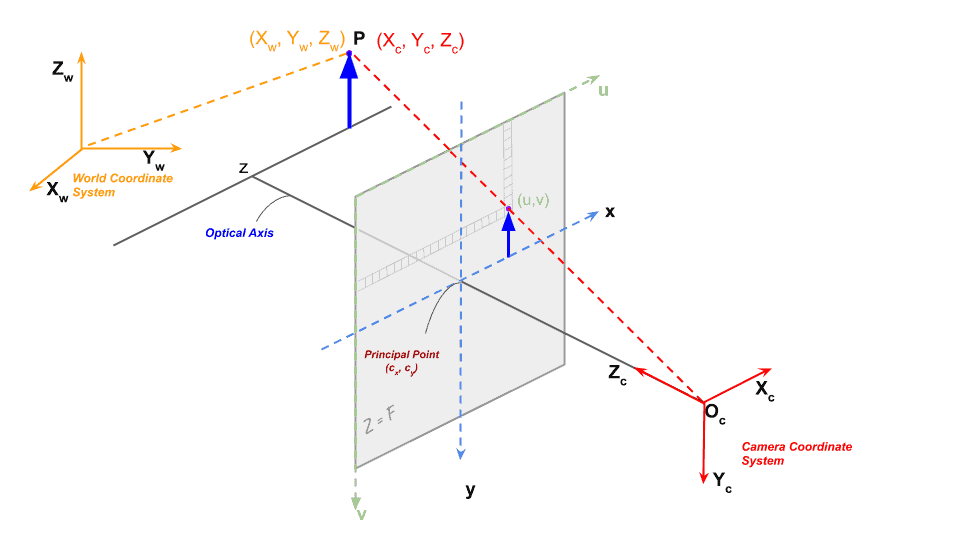
\includegraphics[width=1.0\textwidth]{images/camera-projection-3D-to-2D.png} %插入图片,[]中设置图片大小,{}中是图片文件名
	\caption{世界坐标系到像素坐标系的转换过程,图像来源\href{https://learnopencv.com/geometry-of-image-formation}{LearnOpenCV}}。 %最终文档中希望显示的图片标题
	\label{camera-projection-3D-to-2D} %用于文内引用的标签
\end{figure}

\subsection{世界坐标系到相机坐标系}
如图\ref{camera-projection-3D-to-2D},假设有一个真实三维世界坐标系 $({X_W},{Y_W},{Z_W})$ ,坐标系中的某个点坐标可表示为是 $P({X_W},{Y_W},{Z_W})$。一般情况世界坐标系的原点 $O_W$ 可选择任意位置,比如墙角处等。同理,可以以相机处的物理位置为坐标原点$O_C$得到相机坐标系 $({X_C},{Y_C},{Z_C})$,则同一个世界坐标系下的$P$点相对于相机坐标系的坐标是 $P({X_C},{Y_C},{Z_C})$, 根据相机的小孔成像原理,世界坐标系和相机坐标系下的同一点会在各个坐标方向上存在旋转和平移。


根据\cite{computevision}中公式$(2.24)$可以将两个坐标的旋转和平移表示为:
\begin{equation}\label{cv:rotatin_and_translation}
	x' = Rx + t
\end{equation}
其中$x$和$x'$是两个坐标系下的坐标,$R$是一个 $(3 \times 3)$的标准正交旋转矩阵, $t$是一个$(3 \times 1)$的平移向量。则从世界坐标系到相机坐标系的转换过程可以完整的表示为:
\begin{equation}\label{eq:rotatin_and_translation}
\left[ {\begin{array}{*{20}{c}}
		{{X_C}}\\
		{{Y_C}}\\
		{{Z_C}}
\end{array}} \right] = R \cdot \left[ {\begin{array}{*{20}{c}}
		{{X_W}}\\
		{{Y_W}}\\
		{{Z_W}}
\end{array}} \right] + t = [R|t]\left[ {\begin{array}{*{20}{c}}
		{{X_W}}\\
		{{Y_W}}\\
		{{Z_W}}\\
		1
\end{array}} \right]
\end{equation}
一般情况称旋转矩阵和平移向量的组合 $[R\ |\ t]$ 为外参矩阵(Extrinsic Matrix)。

\subsection{相机坐标系到图像坐标系}
图像坐标系图像所在平面上形成的坐标系,如图以图像中心点为坐标原点(记为$O$),以$x$为横轴,$y$为纵轴的坐标系即图像坐标系,$OO_C$则是相机的焦距$f$。$O_CP$和图像坐标系的交点坐标为$(x,y)$。 则相机坐标系到图像坐标系可以用相似变换得到。如图:
\begin{figure}[H]
	\centering
	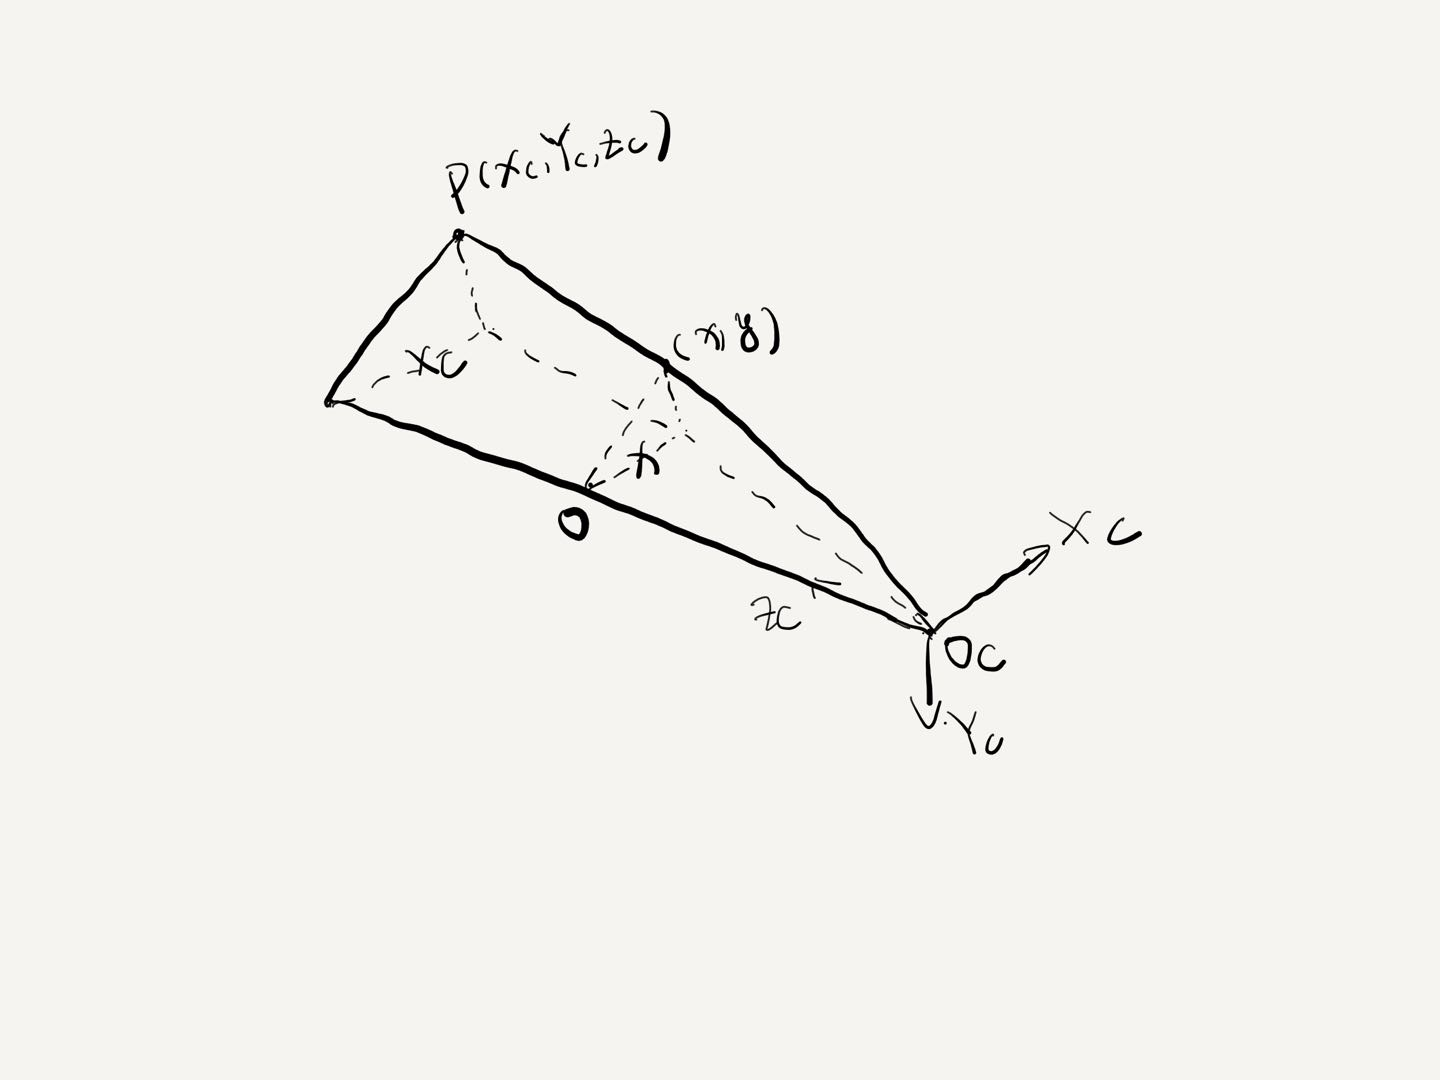
\includegraphics[width=1.0\textwidth]{images/camera_to_image_x.jpg}
	\caption{相机坐标系到图像坐标系x轴变换过程}
	\label{camera-to-image-x}
\end{figure}
由于$Z_C$轴是和图像坐标系垂直的,则根据相似三角形的变换:
\begin{equation}\label{camera_to_image_x}
\frac{x}{{{X_C}}} = \frac{{O{O_C}}}{{{Z_C}}} = \frac{{{f_x}}}{{{Z_C}}}
\end{equation}
同理,对$y$轴有$y={Y_C}{f_y}/{Z_C}$。则从坐标$P({X_C},{Y_C},{Z_C})$到$(x, y)$的变换可以用矩阵表示为:
\begin{equation}\label{camera_to_image_without_translation}
	\left[ {\begin{array}{*{20}{c}}
			{x'}\\
			{y'}\\
			{z'}
	\end{array}} \right] = \left[ {\begin{array}{*{20}{c}}
			{{f_x}}&0&0\\
			0&{{f_y}}&0\\
			0&0&1
	\end{array}} \right]\left[ {\begin{array}{*{20}{c}}
			{{X_C}}\\
			{{Y_C}}\\
			{{Z_C}}
	\end{array}} \right]
\end{equation}
其中$x=x'/z'$, $y=y'/z'$。但是一般的图像平面和相机坐标的位置没有那么标准,可能会存在一定的偏差,偏差来源有两个,一个是$Z_C$坐标轴可能不是刚好通过图像坐标系的坐标原点$O$,两者之间会有一定的偏移,记作$(c_x, c_y)$。另一个是图像平面$x$轴和$y$轴可能存在一定的旋转,不一定是垂直的。对第一种情况,在计算的时候需要考虑偏差,则公式\ref{camera_to_image_x}变成$x + {c_x} = {X_C}\frac{{{f_x}}}{{{Z_C}}}$。这里可能是加上偏差也可能是减去,$c_x$符号则有后续实际计算决定。第二种情况是模型可以简化:
\begin{figure}[H]
	\centering
	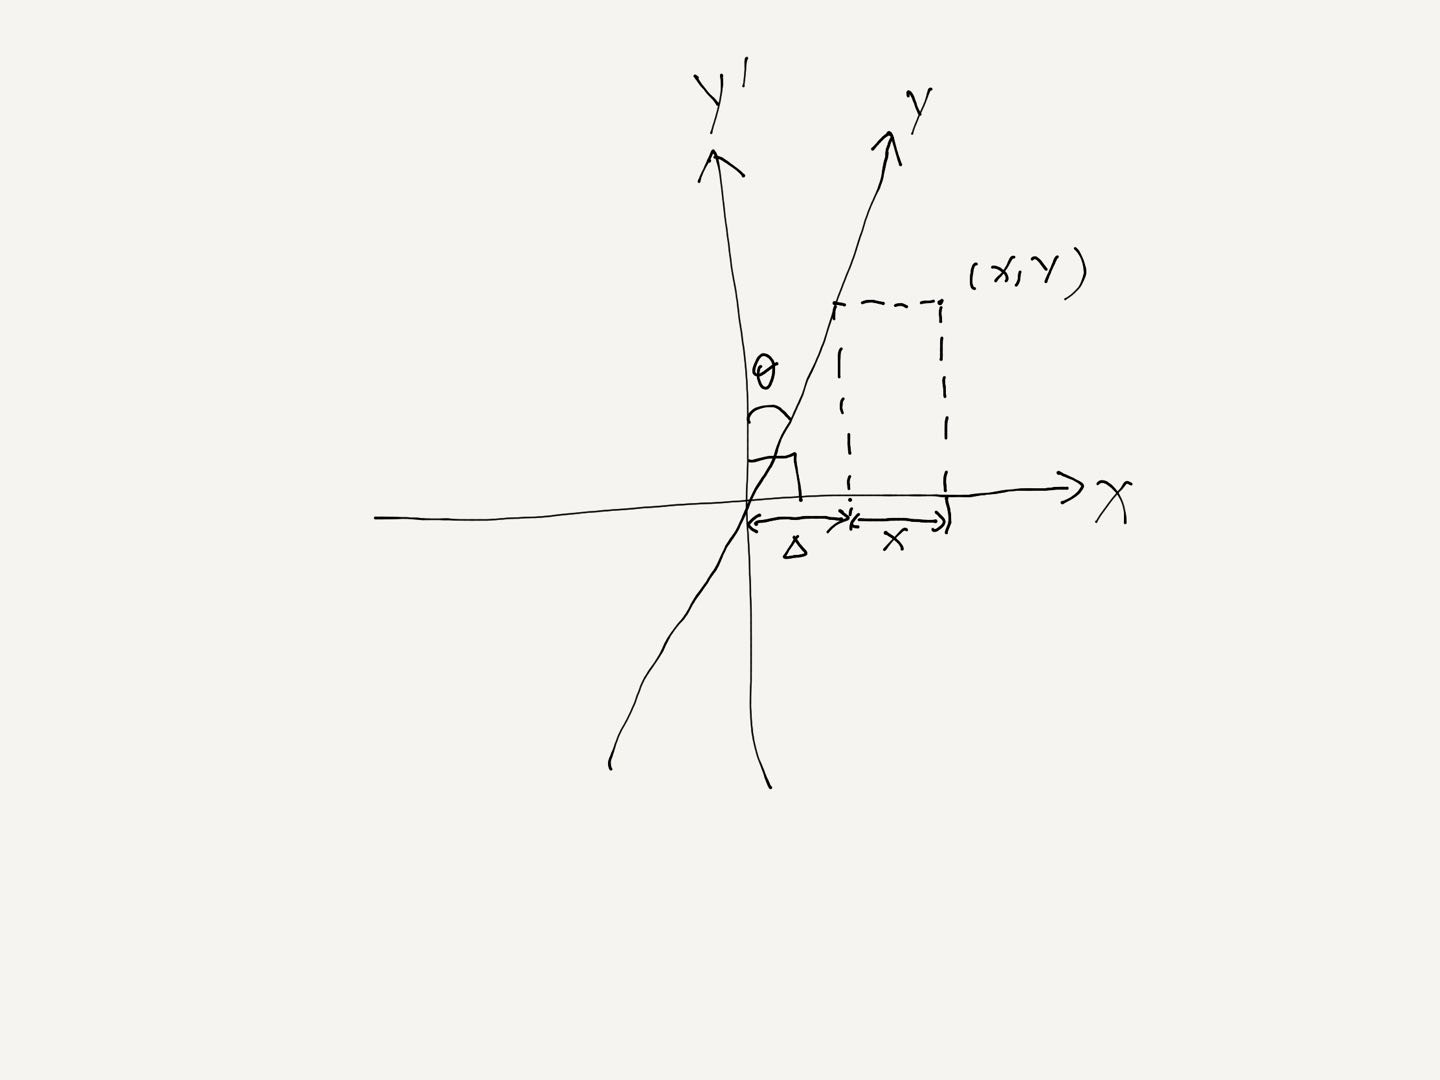
\includegraphics[width=1.0\textwidth]{images/camera_to_image_with_rotation.jpg}
	\caption{x和y轴存在一定的旋转情况}
	\label{camera-to-image-with-rotation}
\end{figure}
假设旋转角度为$\theta $,则公式\ref{camera_to_image_x}变为
\begin{equation}\label{camera_to_image_with_rotation}
\begin{array}{l}
	x = {X_C}\frac{{{f_x}}}{{{Z_C}}} + \Delta  = {X_C}\frac{{{f_x}}}{{{Z_C}}} + \tan (\theta )y\\
	\ \ = {X_C}\frac{{{f_x}}}{{{Z_C}}} + \tan (\theta ){Y_C}\frac{{{f_y}}}{{{Z_C}}}\\
	\ \ = {f_x}\frac{{{X_C}}}{{{Z_C}}} + \gamma \frac{{{Y_C}}}{{{Z_C}}}
\end{array}
\end{equation}
这里因为$\theta$和y轴的焦距$f_y$一般都是固定的,所以用$\gamma$来表示这个常数。结合以上变换最终得到相机坐标系到图像坐标系的变换矩阵为:
\begin{equation}\label{camera_to_image}
\left[ {\begin{array}{*{20}{c}}
		{x'}\\
		{y'}\\
		{z'}
\end{array}} \right] = \left[ {\begin{array}{*{20}{c}}
		{{f_x}}&\gamma &{{c_x}}\\
		0&{{f_y}}&{{c_y}}\\
		0&0&1
\end{array}} \right]\left[ {\begin{array}{*{20}{c}}
		{{X_C}}\\
		{{Y_C}}\\
		{{Z_C}}
\end{array}} \right]
\end{equation}
定义这个变换的矩阵为内参矩阵(Intrinsic Matrix)也称为相机矩阵(camera matrix)。表示为:
\begin{equation}\label{intrinsic_matrix}
K = \left[ {\begin{array}{*{20}{c}}
		{{f_x}}&\gamma &{{c_x}}\\
		0&{{f_y}}&{{c_y}}\\
		0&0&1
\end{array}} \right]
\end{equation}
其中$f_x$和$f_y$分别表示$x$轴和$y$轴上的摄像机焦距。$\gamma$是$x$轴和$y$轴之间的倾斜偏移量,$(c_x, c_y)$是像素坐标中心和相机光学中心轴$Z_C$之间的偏移值。

\subsection{图像坐标到像素坐标}
将图像坐标的坐标原点放在图像的左上角位置则变成了像素坐标,因为一般处理图像时的像素值都是以左上角为原点的。这样的话从$(x, y)$到$(u, v)$像素之间的变换就变成了线性变换:
\begin{equation}\label{pixel_translation}
\begin{array}{l}
	u = x + \frac{W}{2}\\
	v = y + \frac{H}{2}
\end{array}
\end{equation}
其中$(H, W)$表示图像的长宽,也是定值。这样可以对其变换:
\[u = x + \frac{W}{2} = {f_x}\frac{{{X_C}}}{{{Z_C}}} + \gamma \frac{{{Y_C}}}{{{Z_C}}} + {c_x} + \frac{W}{2}\]
由于$c_x$和$W/2$都是常数,可以用一下变化表示新的$c_x$
\[{c_x} \buildrel \Delta \over = {c_x} + \frac{W}{2}\]
这里如果图像坐标系的中心点和$Z_C$轴没有偏差,那么$c_x=0$,则最终得到的内参矩阵中的值$c_x=\frac{W}{2}$。所以一般可以用$W/2$来表示内参值$c_x$。

\subsection{Homography矩阵}
基于以上变化,可以到得到从点$P({X_W},{Y_W},{Z_W})$到像素$(u, v)$的变换过程:
\begin{equation}\label{world_to_pixel}
\begin{array}{l}
	\left[ {\begin{array}{*{20}{c}}
			{u'}\\
			{v'}\\
			{w'}
	\end{array}} \right] = \left[ {\begin{array}{*{20}{c}}
			{{f_x}}&\gamma &{{c_x}}\\
			0&{{f_y}}&{{c_y}}\\
			0&0&1
	\end{array}} \right]\left[ {\begin{array}{*{20}{c}}
			{{X_C}}\\
			{{Y_C}}\\
			{{Z_C}}
	\end{array}} \right]\\
\ \ \ \ \ \ \ \ \ \ = \left[ {\begin{array}{*{20}{c}}
			{{f_x}}&\gamma &{{c_x}}\\
			0&{{f_y}}&{{c_y}}\\
			0&0&1
	\end{array}} \right][R|t]\left[ {\begin{array}{*{20}{c}}
			{{X_W}}\\
			{{Y_W}}\\
			{{Z_W}}
	\end{array}} \right]
\end{array}
\end{equation}

一般为了计算会将世界坐标系的$Z_W$设为0\cite{zhang2000flexible}。则变换矩阵为:
\begin{equation}\label{homography_translation}
\begin{array}{l}
	s\left[ {\begin{array}{*{20}{c}}
			{u'}\\
			{v'}\\
			{w'}
	\end{array}} \right] = \left[ {\begin{array}{*{20}{c}}
			{{f_x}}&\gamma &{{c_x}}\\
			0&{{f_y}}&{{c_y}}\\
			0&0&1
	\end{array}} \right][\begin{array}{*{20}{c}}
		{{r_1}}&{{r_2}}&{{r_3}}&t
	\end{array}]\left[ {\begin{array}{*{20}{c}}
			{{X_W}}\\
			{{Y_W}}\\
			0\\
			1
	\end{array}} \right]\\
	s\left[ {\begin{array}{*{20}{c}}
			u\\
			v\\
			1
	\end{array}} \right] = K[\begin{array}{*{20}{c}}
		{{r_1}}&{{r_2}}&t
	\end{array}]\left[ {\begin{array}{*{20}{c}}
			{{X_W}}\\
			{{Y_W}}\\
			1
	\end{array}} \right]
\end{array}
\end{equation}

其中$r_i$是旋转矩阵的第$i$列,定义homography矩阵为:
\begin{equation}\label{homography}
H = K[R|t]
\end{equation}


对于一般的相机标定,求解内参和外参就可以变换为求解homography矩阵的形式。这里如果可以得到真实世界和像素坐标的对应点作为数据,则可以根据矩阵求解得到homography矩阵的值。但是一般真实世界的坐标不容易测量,常用的方法是使用相同的一个相机对同一个物体拍摄来获取参数,即自我标定的方法\cite{Hartley1994SelfCalibrationFM}。根据\cite{computevision}可知三维坐标系点之间的变换有旋转,平移,仿射变换,投影变换等。其中投影变换(Projective)表示为:
\[x' = Hx\]
其中$x$和$x'$表示变换前后对应的坐标点。$H$被称为透视变换矩阵或者单应性矩阵(perspective transform or homography)。

\subsection{Homography估计}
如果知道坐标点$(x, y, z)$和其经过变换后对应的坐标点$(x', y', z')$。则可以得到homography变换公式:
\begin{equation}\label{homography_two_plane}
\left[ {\begin{array}{*{20}{c}}
		{x'}\\
		{y'}\\
		{z'}two_plane
\end{array}} \right] = \left[ {\begin{array}{*{20}{c}}
		{{H_{11}}}&{{H_{12}}}&{{H_{13}}}\\
		{{H_{21}}}&{{H_{22}}}&{{H_{23}}}\\
		{{H_{31}}}&{{H_{32}}}&{{H_{33}}}
\end{array}} \right]\left[ {\begin{array}{*{20}{c}}
		x\\
		y\\
		z
\end{array}} \right]
\end{equation}

展开矩阵:
\[\frac{{x'}}{{z'}} = \frac{{{H_{11}}x + {H_{12}}y + {H_{13}}z}}{{{H_{31}}x + {H_{32}}y + {H_{33}}z}}\]
一般为了方便计算可以令$z=1$,即图像变换的时候$z$轴可以保持一致。则:
\[x'({H_{31}}x + {H_{32}}y + {H_{33}}) = {H_{11}}x + {H_{12}}y + {H_{13}}\]
\[ - x{H_{11}} - y{H_{12}} - {H_{13}} + 0 + 0 + 0 + x'x{H_{31}} + x'y{H_{32}} + x'{H_{33}} = 0\]
同理得到$y'/z'$的变换展开:
\[0 + 0 + 0 - x{H_{21}} - y{H_{22}} - {H_{23}} + y'x{H_{31}} + y'y{H_{32}} + y'{H_{33}} = 0\]
用矩阵来表示上述变换为:
\begin{equation}\label{homography_estimation}
[\begin{array}{*{20}{c}}
	{ - x}&{ - y}&{ - 1}&0&0&0&{x'x}&{x'y}&{x'}\\
	0&0&0&{ - x}&{ - y}&{ - 1}&{y'x}&{y'y}&{y'}
\end{array}]\left[ {\begin{array}{*{20}{c}}
		{{H_{11}}}\\
		{{H_{12}}}\\
		{{H_{13}}}\\
		{{H_{21}}}\\
		{{H_{22}}}\\
		{{H_{23}}}\\
		{{H_{31}}}\\
		{{H_{32}}}\\
		{{H_{33}}}
\end{array}} \right] = 0
\end{equation}
即:
\[Ah = 0\]
根据线性代数\cite{strang1993introduction}可知这是一个求解线性方程的特征向量问题。求解线性方程即可。常用的方法是将其变成对称矩阵:
\[{A^T}Ah = {A^T}0 = 0\]
然后对其进行$SVD$分解:
\[{A^T}A = U\Sigma {U^T}\]
$U$是正交矩阵,$\Sigma$是奇异值组成的对角矩阵。


\subsection{根据Homography求解旋转矩阵和平移向量}
在相机标定中常用的一种方式是将标定板先选择一个标准位置拍照,然后进行一定的旋转平移拍照。通过几次的图像来计算Homography矩阵。在上一节中可得到计算Homograohy的方法,那如果图像只有旋转和平移,homography的分解方法可参考\cite{malis2007deeper}。

\section{图像处理}
\subsection{滤波}
由于一般拍摄的图像中都含有比较多的噪声,噪声一般是图像上亮度或者颜色值随机变化的信息。比如一个小区域图像像素值都是0,但是其中一个像素值是255,那么这个点就是噪声。平滑(smooth)处理一般就是为了尽可能消除这样的噪声区域,让噪声点部分的像素值不那么明显。一般的方法是:对某一个像素点,求取以这个像素点为中心的局部区域的像素值的加权像素值,然后用新的像素值来代替之前的像素值。这种减小噪声的方法称为滤波(filter)。常见的滤波方式有均值滤波和高斯滤波,均值滤波是在计算新的像素值的时候将区域内的所有像素值求平均,这种操作一般则可以通过卷积的方式来实现,比如:
\begin{figure}[H]
	\centering
	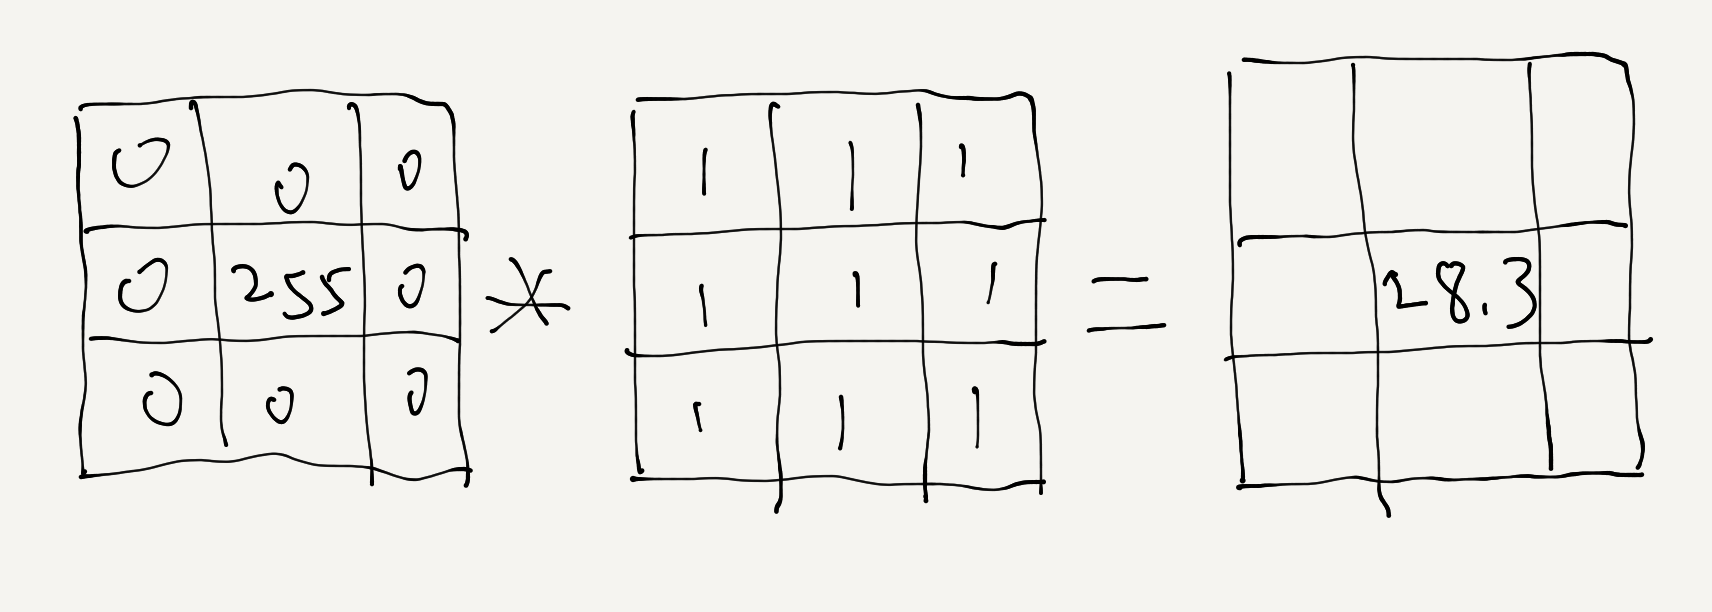
\includegraphics[width=0.7\textwidth]{images/mean-filter.png}
	\caption{均值滤波卷积}
	\label{mean-filter} 
\end{figure}
通过使用一个$3x3$的卷积核对原始图像进行计算,之前的255的像素值就变成了28.3。这样就使得像素值差别没有之前那么明显,整张图像看起开也变得更加平滑。另一种常用的滤波方式是高斯滤波,像均值滤波里使用了全是1的卷积核一样,高斯滤波的区别是使用一个具有高斯分布的卷积核。卷积核的目的主要是作为像素的权重值,那么对于某个点我们一般是希望这个点的权重要比周围像素点权重大的,这样可以尽可能的保留像素的原始信息。而高斯分布则正是中心点概率值大,周围概率值小,所以高斯滤波具有更好的效果。由于图像是二维的,所以一般需要二维高斯分布函数生产一个二维的卷积核。

%%%%%%%%%%%%%%%%%%%%%%%%%%%%%%%%%%%%%%%%%%%%%%%%%%%%%%%%%%%%%%%%%%%%%%%%%%%%%%%%%%%%%%%%%%%%%%%%%%%%%%%%%
\newpage

\fancyhead{}
\fancyhead[CO,CE]{深度学习}

%\setcounter{chapter}{0}
\chapter{第四章\ 深度学习}
本章主要叙述深度学习及机器学习基础及部分网络结构。

\section{机器学习}
\subsection{K-MEAN}
\section{分类模型}
\section{检测模型}
\section{分割模型}

%%%%%%%%%%%%%%%%%%%%%%%%%%%%%%%%%%%%%%%%%%%%%%%%%%%%%%%%%%%%%%%%%%%%%%%%%%%%%%%%%%%%%%%%%%%%%%%%%%%%%%%%%
\newpage

\fancyhead{}
\fancyhead[CO,CE]{算法}

%\setcounter{chapter}{0}
\chapter{第五章\ 算法}

%%%%%%%%%%%%%%%%%%%%%%%%%%%%%%%%%%%%%%%%%%%%%%%%%%%%%%%%%%%%%%%%%%%%%%%%%%%%%%%%%%%%%%%%%%%%%%%%%%%%%%%%%
\newpage

\fancyhead{}
\fancyhead[CO,CE]{计算机基础}

%\setcounter{chapter}{0}
\chapter{第六章\ 计算机基础}
\section{基础概念}
\subsection{程序编译原理}
程序编译步骤包括:
 \begin{center} 源文件 $\rightarrow$ 预处理器 $\rightarrow$ 编译器 $\rightarrow$ 连接器 $\rightarrow$ 目标机器代码 \end{center}
预处理器: 完成将多个源文件汇聚在一起的任务,主要包括将头文件代码copy到源文件中,将对应的宏进去扩展开。\\
编译器: 完成预处理后文件到汇编语言的转换。(编译器包括语法分析、代码生成等步骤)\\
汇编器: 将汇编程序生成可重定位的机器代码。\\
链接器: 将多个编译文件链接在一起。\\
\subsection{BandWidth}
\section{常用命令工具}
\subsection{Windows}
\subsection{Ubuntu}
\textbf{创建虚拟环境}
\begin{lstlisting}[language=bash]
# virtualenv
which python3.7
virtualenv venv -p /usr/bin/python3.7
\end{lstlisting}

%%%%%%%%%%%%%%%%%%%%%%%%%%%%%%%%%%%%%%%%%%%%%%%%%%%%%%%%%%%%%%%%%%%%%%%%%%%%%%%%%%%%%%%%%%%%%%%%%%%%%%%%%
\newpage

\fancyhead{}
\fancyhead[CO,CE]{c++}

%\setcounter{chapter}{0}
\chapter{第七章\ c++}

\section{基础概念}

\subsection{类型别名}
类型别名(type alias)可以使用关键字typedef或者using,用来表示将某个类型重命名。
\begin{lstlisting}
typedef type new_name;
using new_name = type;
\end{lstlisting}

\subsection{typename}
在模板声明的模板参数列表中,typename可以替代class来声明类型模板参数和模板模板参数。
\begin{lstlisting}
template <typename T>
\end{lstlisting}
在模板内,如果要使用一个依赖于模板参数的类型,则需要用typename来说明,参考c++标准:A name used in a template declaration or definition and that is dependent on a template-parameter is assumed not to name a type unless the applicable name lookup finds a type name or the name is qualified by the keyword typename。
\begin{lstlisting}
template <typename T>
struct A {
  typedef typename T::Type type;
};
\end{lstlisting}
这里要使用模板参数T的一个类型Type并用typedef将其命名为type。但是由于是一个依赖类型(Dependent names),即Type依赖传入的模板参数T。但是T是一个未知的类型,所以是不清楚Type的具体含义的,比如是类型还是静态成员变量什么的。所以需要加上typename来修饰让编译清楚这是一个数据类型,从而编译时才不会出错。

\subsection{函数原型}
函数原型( function prototype)是函数的声明,它告诉程序函数返回值的类型以及参数的数量和类型。函数类型需要在头文件中进行定义然后在cpp文件中实现函数定义。函数原型中的名字是可选的可以省略,即参数的名字是可以省略的。
\begin{lstlisting}
void fun(int a);
void fun(int);
void fun(int a = 1);
\end{lstlisting}

\subsection{namespace}
\begin{lstlisting}
namespace {}
\end{lstlisting}

\subsection{decltype}
\subsection{extern}
\subsection{函数指针}
\subsection{noexcept}
\subsection{restrict}
\subsection{value initialization}

\section{内存管理}
\subsection{基本内存概念}
计算机以bit序列来存储数据,每个bit(比特)表示非0即1。大多数计算机以2的整数次幂个bit作为块来处理内存,可寻址的最小内存块称为"字节"(byte),一个字节含有8bit的内存大小,计算机中将内存中每个字节和一个数字(称为地址,address)进行关联。
1 byte = 8 bit, 1 K = 1024 byte, 1 M = 1024 K, 1 G = 1024 M, 1 KB = 1000 byte。c++中所有的数据类型都是以字节为基础单位的,常用数据类型字节大小: bool(1字节), char(1字节), int(4字节), double(8字节)。
\subsection{const}
\subsection{heap}
\subsection{stack}
\subsection{Free Store}
\subsection{Global/Static}

\section{class}
\begin{lstlisting}
class derived_class : final base_class {
 public:
  derived_class() = default;
  derived_class & operator =( const derived_class & ) = delete;
  
  virtual void methods() final;	 //
};
\end{lstlisting}

\subsection{default}
类中的default关键字表示应该默认使用default部分定义的函数方法。当在class中定义某个方法为default属性时,编译器会自动为该方法创建一个对应的函数体实例化,不需要手动的来实现对应的函数内容,这在部分构造函数定义中十分有用,比如需要定义一套拷贝构造和赋值构造函数,一般的拷贝构造时比较麻烦的需要处理类里所有的成员变量等,但是使用default的话就可以让编译器默认来实现。
\begin{lstlisting}
class A {
 public:
  A(const A& rhs) = default;  // copy construct
  bool operator ==( const & A ) = default;
  bool operator !=( const & A ) = default;
  
 private:
  int data_;
};

// default same as:
A(const A& rhs) : data_(rhs.data_) {}

A aa;
auto a = aa;  // copy construct and initialize class a
\end{lstlisting}
拷贝构造是使用其他对象的值来初始化当前对象。注意是初始化类的时候对应等号左边的类是在拷贝构造的时候完成初始化的。赋值构造则是直接用一个新的对象来替换当前对象,赋值构造在调用的时候等号前后两个类都已经初始化完了,赋值构造完成赋值替换。
\begin{lstlisting}
class A {
 public:
  A& operator=(const A& rhs) = default;  // assignment construct

 private:
  int data_;
};
	
// default same as:
A& operator=(const A& rhs) {data_ = rhs.data_; return *this;}
	
A aa, a;  // a and aa already initialized.
a = aa;  // assignment construct
\end{lstlisting}

\subsection{delete}
类中使用delete修饰表示禁用对应的方法,编译器也不会自动实现对应的方法。使用delete的好处是在编译期就可以对代码进行规范性检查,如果有其他地方调用了delete的方法则会在编译器出错而不是到运行时出错。delete常用的是禁用拷贝构造:
\begin{lstlisting}
struct type {
 type & operator =( const type & ) = delete;
 type( const type & ) = delete;
};
\end{lstlisting}

使用delete完成模板的特化:
\begin{lstlisting}
// Delete primary class template, allow specializations
template<typename>
struct s = delete;
template<>
struct s<int> {
};

// Delete class specialization
template<typename>
struct t {
};

template<>
struct t<int> = delete;
\end{lstlisting}

使用delete来修饰析构函数,这种情况其实有点怪,因为一单析构函数被delete关键字修饰则对应的类不能够被析构掉。修饰析构函数一般是为了防止类中有申请的自由存储的内存等没有被释放的情况。比如:
\begin{lstlisting}
struct data {
  //...
};
	
struct data_protected {
 ~data_protected() = delete;
 data d;
};
struct data_factory {		
  ~data_factory() {
  for (data* d : data_container) {
	// this is safe, because no one can call 'delete' on d
	delete d;
	}
  }
		
  data_protected* createData() {
	data* d = new data();
	data_container.push_back(d);
	return (data_protected*)d;
  }

  std::vector<data*> data_container;
};
\end{lstlisting}

这里对结构体data\_protected,里面的data属性由于是new出来的,我们希望在特定的情况外部控制其释放。这样的话就最好禁用data\_protedted的析构函数使其一致存成,否则可能无法访问到对应的data成员。所以一般如果希望外部用户来控制对象的生命周期的话可以用delete。但是坏处是对应的类会一直存在。

\subsection{final}
\subsection{explicit}

\subsection{virtual}
\subsection{虚函数表}
\section{模板}
template代码的位置不能在.cpp/.cc之中,Templated code implementation should never be in a .cpp file: your compiler has to see them at the same time as it sees the code that calls them.一般都是放在.h文件中. 如果希望放在.cpp文件中要对class进行 explicit instantiation,对类模板A在.cpp最后加上:template class A;来实现显示生成object. 不能在class中特化模板;模板的定义一般是放在.h中,但是对该模板的特化定义要放在.cpp函数中.否则会有重定义的问题。模板只是代码的简化和宏展开一个效果,编译器会对每个类型都增加一个实现。不要在template中对某个特殊类型进行不同逻辑的处理,如果需要这样请特化。

\subsection{可选模板参数}
分析:
\begin{lstlisting}
template <typename T>
struct FUN {
	typedef int Type;
	...
}

template <typename T, typename = typename FUN<T>::Type>
void fun();
\end{lstlisting}
模板fun有两个模板参数一个是T另一个是typename = typename FUN<T>::Type,根据typename的Dependent names含义可以将fun简化为:
\begin{lstlisting}
template <typename T, typename = int>
void fun();
\end{lstlisting}
这里typename = 表示declaring template type parameters, 即需要定义一个模板变量。类模板定义的时候是可以指定一个默认值的。同时由于函数声明的时候函数名字可以省略,所以模板的第二个参数即定义了一个参数名字省略的int类型值。可以等价于:
\begin{lstlisting}
template <typename T, typename Type = int>
void fun();
	
template <typename T, int>
void fun();
\end{lstlisting}
这里用Type表示省略的名字,实际上相当于实现了一个偏特化的类,第二个模板参数是int。

\subsection{可变参数模板}

%% section for std
\section{std}
\subsection{std::vector}
\subsection{std::forward}
\subsection{std::enable\_if}
\subsection{std::find\_if}

%% section for cmake
\section{cmake}
\subsection{cmake demo}
\section{设计模式}
%%%%%%%%%%%%%%%%%%%%%%%%%%%%%%%%%%%%%%%%%%%%%%%%%%%%%%%%%%%%%%%%%%%%%%%%%%%%%%%%%%%%%%%%%%%%%%%%%%%%%%%%%
%%  参考文献  %%
\newpage
 
\fancyhead{}
\fancyhead[CO,CE]{参考文献}
 
\bibliographystyle{plain}
 
\chapter{参考文献}
\bibliography{reference.bib}

 
\end{document}